\documentclass[10pt,a4paper]{article}
\usepackage[T1]{fontenc}
\usepackage{lmodern}
\usepackage[margin=1.7cm]{geometry}
\usepackage{amsmath,amssymb}
\usepackage{xcolor}
\usepackage{graphicx}
\usepackage{tikz}
\usetikzlibrary{positioning,arrows.meta,fit,backgrounds,calc,shapes.multipart}
\usepackage{tabularx,booktabs,array}
\usepackage[colorlinks=true,linkcolor=blue!50!black]{hyperref}

\setlength{\parindent}{0pt}
\setlength{\parskip}{4pt}

% ---------- helpers ----------
\newcommand{\code}[1]{\texttt{\detokenize{#1}}}
\newcommand{\fnn}[1]{\textbf{\texttt{\detokenize{#1}}}}
\newcommand{\task}[1]{\hfill{\scriptsize\sffamily\bfseries\textcolor{orange!75!black}{Task #1}}}
\newcommand{\given}{{\scriptsize\sffamily\textcolor{black!55}{provided}}}

\definecolor{todo}{RGB}{255,236,214}
\definecolor{tododraw}{RGB}{204,110,20}

\tikzset{
  arr/.style={-{Stealth[length=2.2mm]}, thick, black!65},
  fn/.style={draw=black!50, fill=black!4, rounded corners=2pt, text width=6.6cm,
             align=left, inner sep=4pt, font=\small},
  todo/.style={fn, draw=tododraw, fill=todo, line width=0.8pt},
  outn/.style={font=\footnotesize, text width=6.3cm, align=left, text=blue!40!black},
  file/.style={draw=black!45, fill=white, font=\footnotesize\ttfamily, inner sep=3pt,
               minimum height=6mm},
  store/.style={draw=blue!50!black, fill=blue!6, font=\footnotesize, inner sep=3pt,
                align=center},
  stage/.style={draw=#1!55!black, fill=#1!5, rounded corners=5pt, inner sep=7pt},
  stagelbl/.style={font=\small\bfseries\sffamily, text=#1!45!black, anchor=south west},
}

\title{\textbf{Lab 02 -- How the Code Fits Together}\\[2pt]
\large Structure from Motion \& RANSAC line fitting}
\author{}
\date{}

\begin{document}
\maketitle
\vspace{-1.2cm}

\section*{How to read this document}
\begin{itemize}
  \setlength{\itemsep}{1pt}
  \item The SfM part has \textbf{one class} (\code{Image}). Everything else is
        \textbf{plain functions} that pass NumPy arrays, dicts and \code{Image} objects around.
        \code{sfm.py} is the script that calls them in order.
  \item Grey boxes are \given\ code. \colorbox{todo}{Orange boxes} contain a TODO and are
        labelled with the task number from the handout.
  \item Blue text next to a box is what that step \emph{produces}, with array shapes.
        $N$ = number of 3D points, $M$ = number of matches, $K_i$ = number of keypoints in image $i$.
  \item Run \code{sfm.py} from inside \code{code/}: it loads data from the relative path \code{../data}.
\end{itemize}

\tableofcontents

% =====================================================================
\clearpage
\section{The big picture: what \texttt{sfm.py} does}
\label{sec:pipeline}

\code{main()} in \code{sfm.py} runs in four stages: \textbf{load} the data,
\textbf{initialize} the map from two images, \textbf{extend} it one image at a time, and
\textbf{plot} the result. Stage C only runs when \code{run_map_extension = True}.

\begin{center}
\resizebox{!}{0.84\textheight}{%
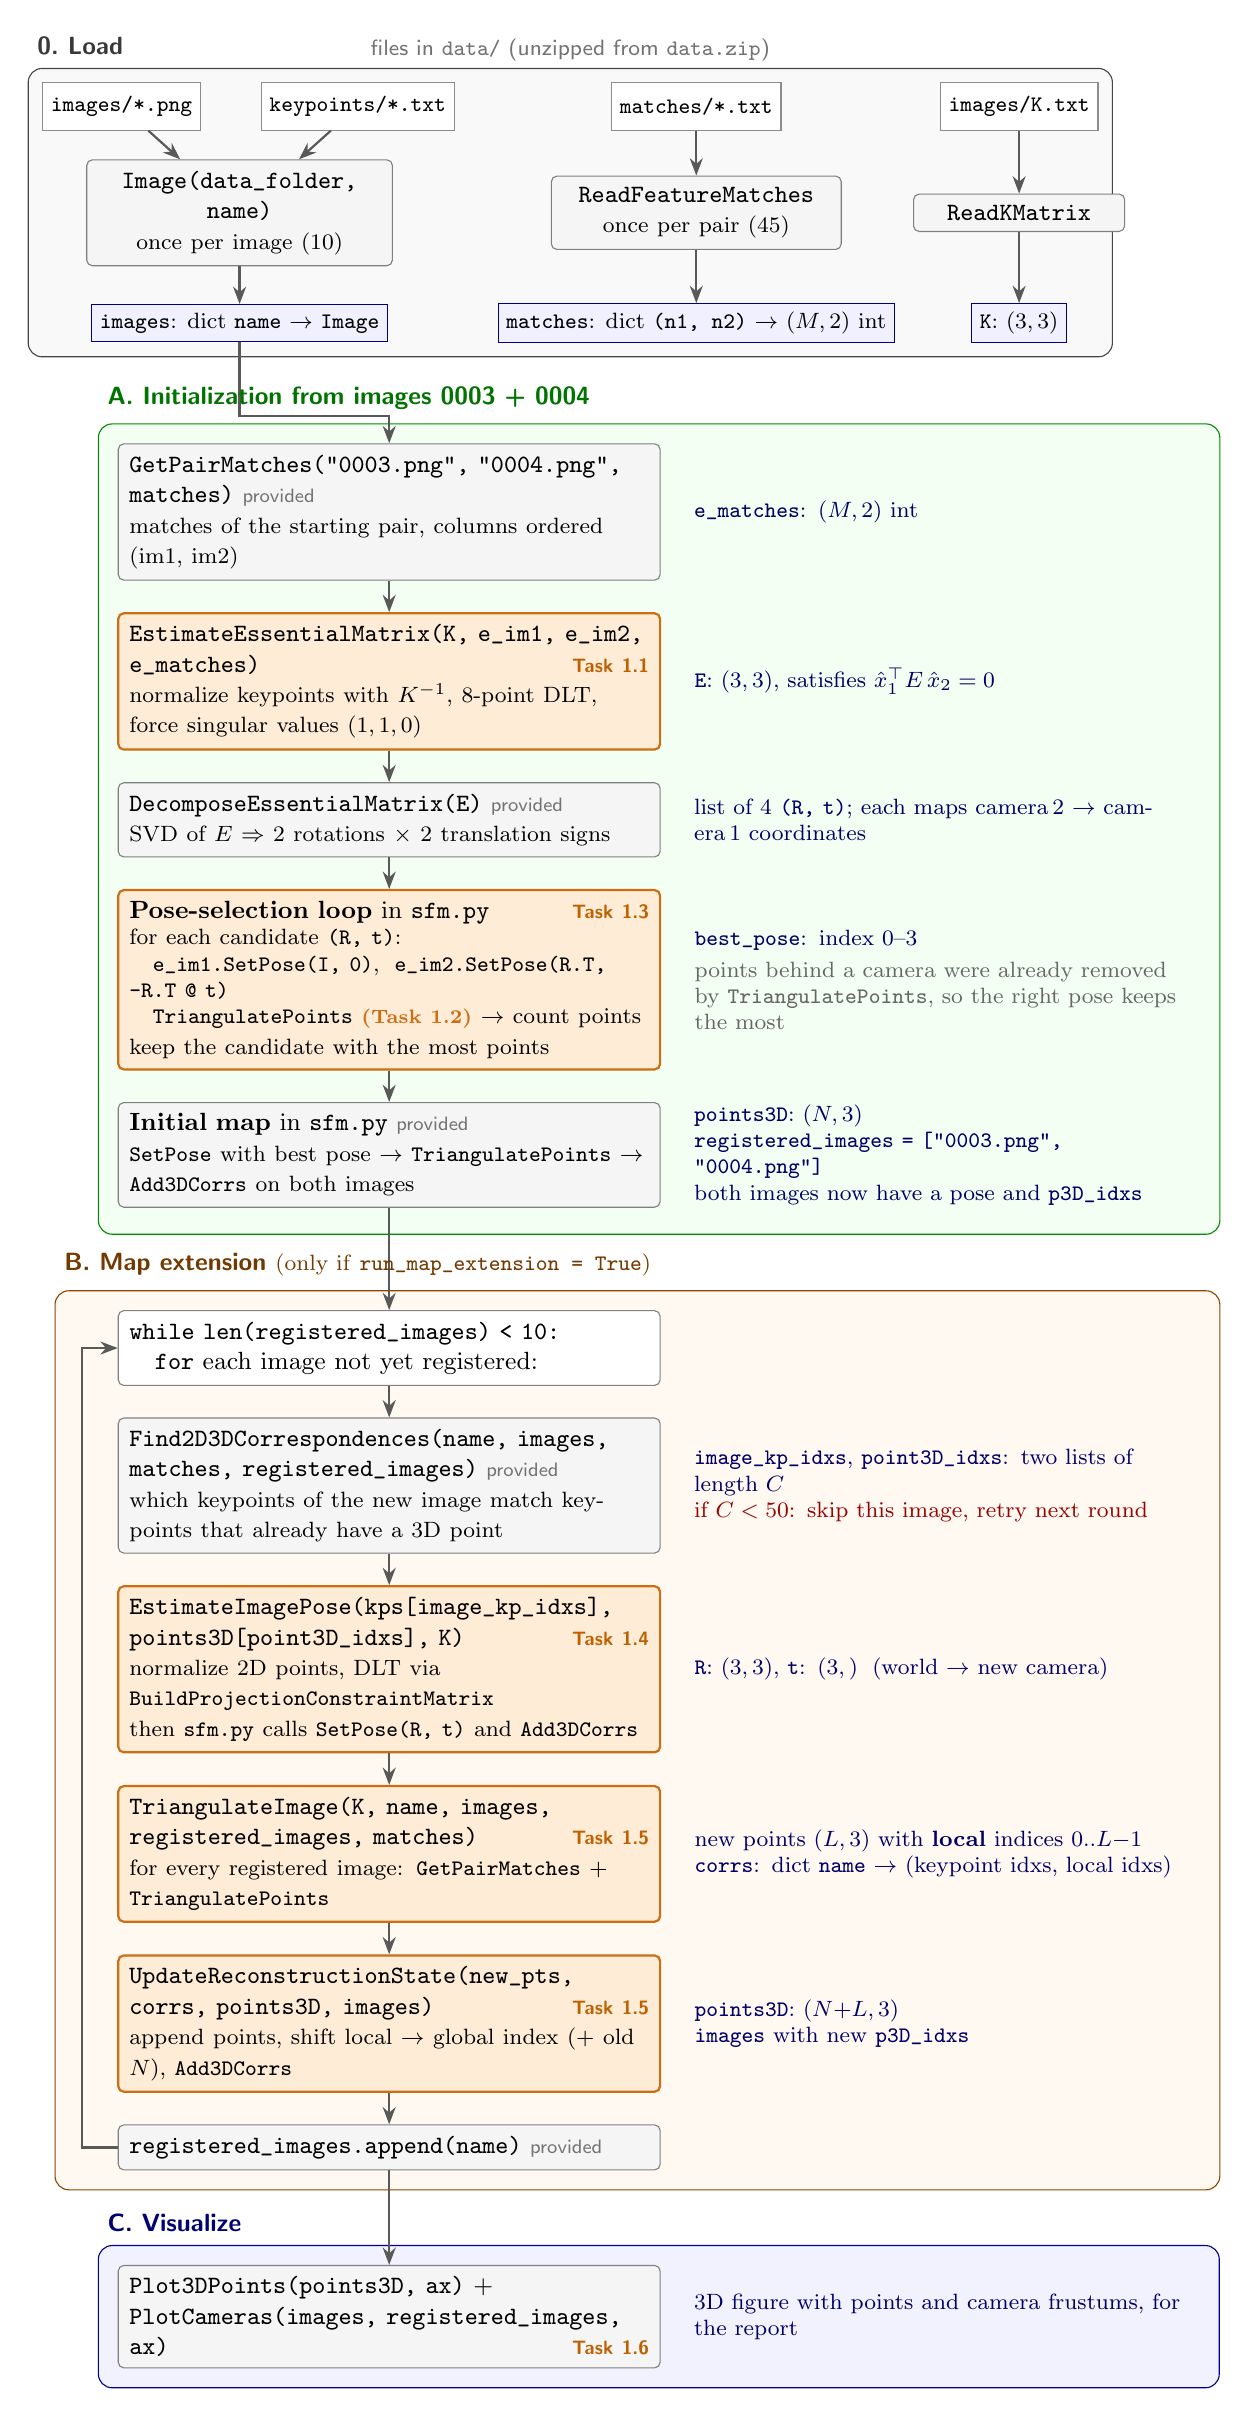
\begin{tikzpicture}[node distance=4mm]

% ---------------- data files ----------------
\node[file] (fimg) at (-6.0,0) {images/*.png};
\node[file] (fkp)  at (-3.0,0) {keypoints/*.txt};
\node[file] (fmt)  at ( 1.3,0) {matches/*.txt};
\node[file] (fK)   at ( 5.4,0) {images/K.txt};
\node[font=\footnotesize\sffamily, text=black!55, anchor=south] at (-0.3,0.45)
     {files in \texttt{data/} (unzipped from \texttt{data.zip})};

% ---------------- loaders ----------------
\node[fn, text width=3.6cm, align=center] (ldimg) at (-4.5,-1.35)
     {\fnn{Image(data_folder, name)}\\{\footnotesize once per image (10)}};
\node[fn, text width=3.4cm, align=center] (ldmt) at (1.3,-1.35)
     {\fnn{ReadFeatureMatches}\\{\footnotesize once per pair (45)}};
\node[fn, text width=2.4cm, align=center] (ldK) at (5.4,-1.35) {\fnn{ReadKMatrix}};
\draw[arr] (fimg) -- (ldimg);
\draw[arr] (fkp)  -- (ldimg);
\draw[arr] (fmt)  -- (ldmt);
\draw[arr] (fK)   -- (ldK);

% ---------------- in-memory stores ----------------
\node[store] (simg) at (-4.5,-2.75) {\code{images}: dict \code{name} $\to$ \code{Image}};
\node[store] (smt)  at ( 1.3,-2.75) {\code{matches}: dict \code{(n1, n2)} $\to$ $(M,2)$ int};
\node[store] (sK)   at ( 5.4,-2.75) {\code{K}: $(3,3)$};
\draw[arr] (ldimg) -- (simg);
\draw[arr] (ldmt)  -- (smt);
\draw[arr] (ldK)   -- (sK);

\begin{scope}[on background layer]
  \node[stage=gray, fit=(fimg)(fK)(simg)(smt)(sK)(ldimg), inner sep=5pt] (stage0) {};
\end{scope}
\node[stagelbl=gray] at ($(stage0.north west)+(0,0.05)$) {0.\ Load};

% ---------------- stage A ----------------
\node[fn] (a1) at (-2.6,-5.15)
  {\fnn{GetPairMatches}\code{("0003.png", "0004.png", matches)} \given\\
   {\footnotesize matches of the starting pair, columns ordered (im1, im2)}};
\node[outn, right=3mm of a1] (a1o) {\code{e_matches}: $(M,2)$ int};

\node[todo, below=of a1] (a2)
  {\fnn{EstimateEssentialMatrix}\code{(K, e_im1, e_im2, e_matches)} \task{1.1}\\
   {\footnotesize normalize keypoints with $K^{-1}$, 8-point DLT, force singular values $(1,1,0)$}};
\node[outn, right=3mm of a2] (a2o) {\code{E}: $(3,3)$, satisfies $\hat{x}_1^\top E\, \hat{x}_2 = 0$};

\node[fn, below=of a2] (a3)
  {\fnn{DecomposeEssentialMatrix}\code{(E)} \given\\
   {\footnotesize SVD of $E$ $\Rightarrow$ 2 rotations $\times$ 2 translation signs}};
\node[outn, right=3mm of a3] (a3o)
  {list of 4 \code{(R, t)}; each maps camera\,2 $\to$ camera\,1 coordinates};

\node[todo, below=of a3] (a4)
  {\textbf{Pose-selection loop} in \code{sfm.py} \task{1.3}\\
   {\footnotesize for each candidate \code{(R, t)}:\\
   \quad \code{e_im1.SetPose(I, 0)},\; \code{e_im2.SetPose(R.T, -R.T @ t)}\\
   \quad \fnn{TriangulatePoints} \textcolor{tododraw}{\scriptsize\bfseries(Task 1.2)} $\to$ count points\\
   keep the candidate with the most points}};
\node[outn, right=3mm of a4] (a4o)
  {\code{best_pose}: index 0--3\\[2pt]
   {\color{black!60} points behind a camera were already removed by \code{TriangulatePoints}, so the right pose keeps the most}};

\node[fn, below=of a4] (a5)
  {\textbf{Initial map} in \code{sfm.py} \given\\
   {\footnotesize \code{SetPose} with best pose $\to$ \fnn{TriangulatePoints} $\to$ \code{Add3DCorrs} on both images}};
\node[outn, right=3mm of a5] (a5o)
  {\code{points3D}: $(N,3)$\\
   \code{registered_images = ["0003.png", "0004.png"]}\\
   both images now have a pose and \code{p3D_idxs}};

\draw[arr] (simg.south) |- ($(a1.north)+(0,0.35)$) -- (a1.north);
\draw[arr] (a1) -- (a2);
\draw[arr] (a2) -- (a3);
\draw[arr] (a3) -- (a4);
\draw[arr] (a4) -- (a5);

\begin{scope}[on background layer]
  \node[stage=green, fit=(a1)(a1o)(a5)(a5o)(a4o)] (stageA) {};
\end{scope}
\node[stagelbl=green] at ($(stageA.north west)+(0,0.05)$)
  {A.\ Initialization from images 0003 + 0004};

% ---------------- stage B ----------------
\node[fn, fill=white, below=13mm of a5] (b0)
  {\code{while len(registered_images) < 10:}\\
   \quad \code{for} each image not yet registered:};

\node[fn, below=of b0] (b1)
  {\fnn{Find2D3DCorrespondences}\code{(name, images, matches, registered_images)} \given\\
   {\footnotesize which keypoints of the new image match keypoints that already have a 3D point}};
\node[outn, right=3mm of b1] (b1o)
  {\code{image_kp_idxs}, \code{point3D_idxs}: two lists of length $C$\\
   {\color{red!60!black} if $C < 50$: skip this image, retry next round}};

\node[todo, below=of b1] (b2)
  {\fnn{EstimateImagePose}\code{(kps[image_kp_idxs], points3D[point3D_idxs], K)} \task{1.4}\\
   {\footnotesize normalize 2D points, DLT via \code{BuildProjectionConstraintMatrix}}\\
   {\footnotesize then \code{sfm.py} calls \code{SetPose(R, t)} and \code{Add3DCorrs}}};
\node[outn, right=3mm of b2] (b2o) {\code{R}: $(3,3)$, \code{t}: $(3,)$ \;(world $\to$ new camera)};

\node[todo, below=of b2] (b3)
  {\fnn{TriangulateImage}\code{(K, name, images, registered_images, matches)} \task{1.5}\\
   {\footnotesize for every registered image: \code{GetPairMatches} + \code{TriangulatePoints}}};
\node[outn, right=3mm of b3] (b3o)
  {new points $(L,3)$ with \textbf{local} indices $0..L{-}1$\\
   \code{corrs}: dict \code{name} $\to$ (keypoint idxs, local idxs)};

\node[todo, below=of b3] (b4)
  {\fnn{UpdateReconstructionState}\code{(new_pts, corrs, points3D, images)} \task{1.5}\\
   {\footnotesize append points, shift local $\to$ global index (+ old $N$), \code{Add3DCorrs}}};
\node[outn, right=3mm of b4] (b4o)
  {\code{points3D}: $(N{+}L,3)$\\ \code{images} with new \code{p3D_idxs}};

\node[fn, below=of b4] (b5) {\code{registered_images.append(name)} \given};

\draw[arr] (a5) -- (b0);
\draw[arr] (b0) -- (b1);
\draw[arr] (b1) -- (b2);
\draw[arr] (b2) -- (b3);
\draw[arr] (b3) -- (b4);
\draw[arr] (b4) -- (b5);
\draw[arr] (b5.west) -- ++(-0.45,0) |- (b0.west);

\begin{scope}[on background layer]
  \node[stage=orange, fit={(b0)(b1o)(b5)(b4o)($(b5.west)+(-0.55,0)$)}] (stageB) {};
\end{scope}
\node[stagelbl=orange] at ($(stageB.north west)+(0,0.05)$)
  {B.\ Map extension \normalfont\footnotesize(only if \code{run_map_extension = True})};

% ---------------- stage C ----------------
\node[fn, below=12mm of b5] (c1)
  {\fnn{Plot3DPoints}\code{(points3D, ax)} + \fnn{PlotCameras}\code{(images, registered_images, ax)} \task{1.6}};
\node[outn, right=3mm of c1] (c1o) {3D figure with points and camera frustums, for the report};
\draw[arr] (b5) -- (c1);

\begin{scope}[on background layer]
  \node[stage=blue, fit=(c1)(c1o)] (stageC) {};
\end{scope}
\node[stagelbl=blue] at ($(stageC.north west)+(0,0.05)$) {C.\ Visualize};

\end{tikzpicture}}

{\small\itshape The full SfM pipeline in \code{sfm.py}. \code{K}, \code{images} and \code{matches}
are used by almost every step, so only the first arrow out of Stage 0 is drawn.}
\end{center}

% =====================================================================
\clearpage
\section{Files and who imports whom}

\begin{figure}[h!]
\centering
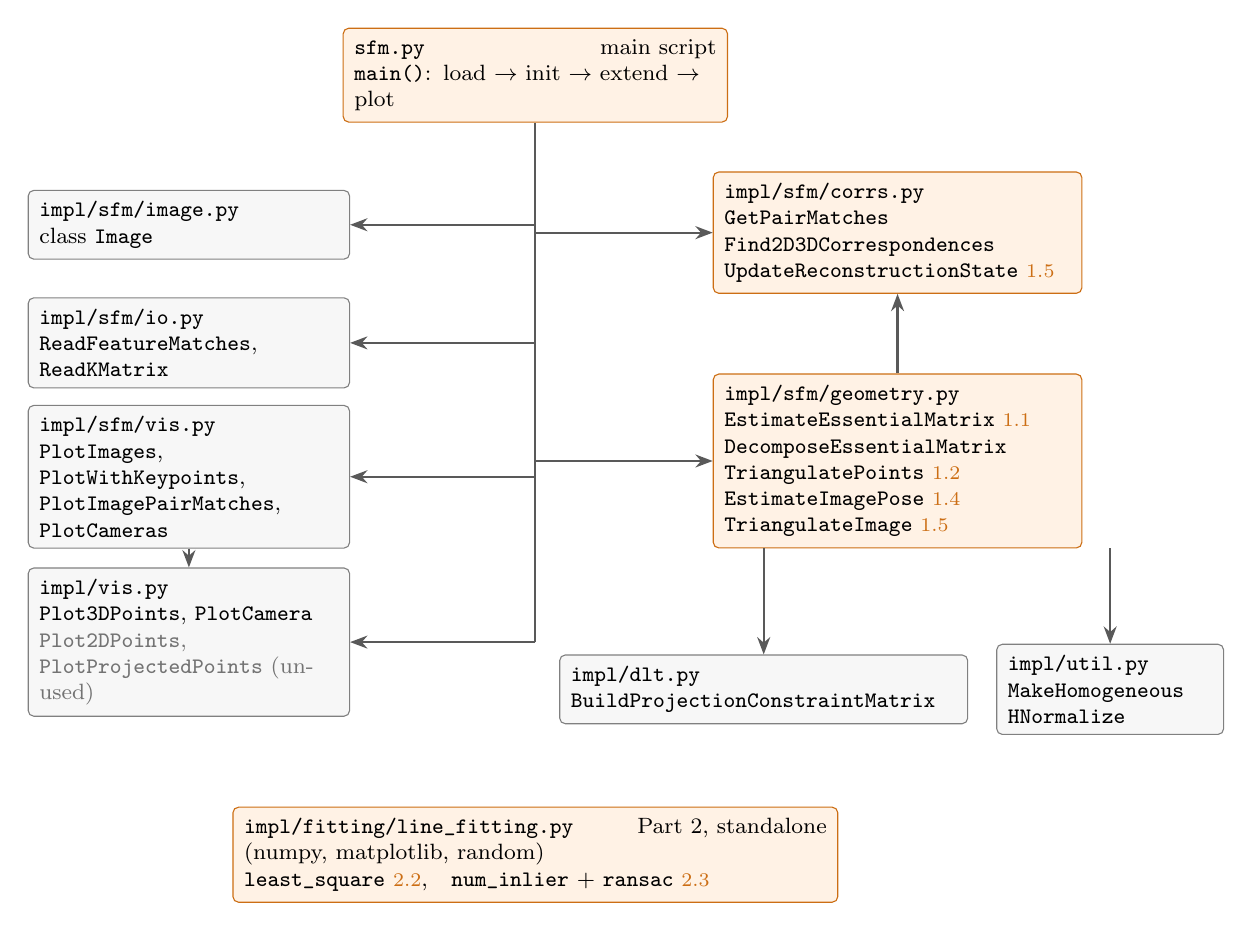
\begin{tikzpicture}[
  mod/.style={draw=black!50, fill=black!3, rounded corners=2pt, align=left,
              font=\footnotesize, inner sep=4pt, text width=#1},
  mod/.default=3.8cm,
  tmod/.style={mod=#1, fill=orange!10, draw=tododraw},
  tmod/.default=3.8cm]

\node[tmod=4.6cm] (sfm) at (0,0)
  {\textbf{\code{sfm.py}} \hfill main script\\
   \code{main()}: load $\to$ init $\to$ extend $\to$ plot};

% left column
\node[mod] (image) at (-4.4,-1.9) {\textbf{\code{impl/sfm/image.py}}\\ class \code{Image}};
\node[mod] (io)    at (-4.4,-3.4) {\textbf{\code{impl/sfm/io.py}}\\ \code{ReadFeatureMatches}, \code{ReadKMatrix}};
\node[mod] (svis)  at (-4.4,-5.1) {\textbf{\code{impl/sfm/vis.py}}\\ \code{PlotImages}, \code{PlotWithKeypoints},\\
   \code{PlotImagePairMatches}, \code{PlotCameras}};
\node[mod] (vis)   at (-4.4,-7.2) {\textbf{\code{impl/vis.py}}\\ \code{Plot3DPoints}, \code{PlotCamera}\\
   {\color{black!55}\code{Plot2DPoints}, \code{PlotProjectedPoints} (unused)}};

% right column
\node[tmod=4.4cm] (corrs) at (4.6,-2.0)
  {\textbf{\code{impl/sfm/corrs.py}}\\ \code{GetPairMatches}\\ \code{Find2D3DCorrespondences}\\
   \code{UpdateReconstructionState} \textcolor{tododraw}{\scriptsize 1.5}};
\node[tmod=4.4cm] (geom) at (4.6,-4.9)
  {\textbf{\code{impl/sfm/geometry.py}}\\
   \code{EstimateEssentialMatrix} \textcolor{tododraw}{\scriptsize 1.1}\\
   \code{DecomposeEssentialMatrix}\\
   \code{TriangulatePoints} \textcolor{tododraw}{\scriptsize 1.2}\\
   \code{EstimateImagePose} \textcolor{tododraw}{\scriptsize 1.4}\\
   \code{TriangulateImage} \textcolor{tododraw}{\scriptsize 1.5}};
\node[mod=4.9cm] (dlt)  at (2.9,-7.8) {\textbf{\code{impl/dlt.py}}\\ \code{BuildProjectionConstraintMatrix}};
\node[mod=2.6cm] (util) at (7.3,-7.8) {\textbf{\code{impl/util.py}}\\ \code{MakeHomogeneous}\\ \code{HNormalize}};

% bus from sfm.py
\draw[thick, black!65] (sfm.south) -- (0,-7.2);
\foreach \n in {image, io, svis, vis} \draw[arr] (0,0 |- \n.east) -- (\n.east);
\foreach \n in {corrs, geom} \draw[arr] (0,0 |- \n.west) -- (\n.west);
\draw[arr] (svis) -- (vis);
\draw[arr] (geom.north) -- (corrs.south);
\draw[arr] (geom.south -| dlt.north) -- (dlt.north);
\draw[arr] (geom.south -| util.north) -- (util.north);

\node[tmod=7.4cm] (lf) at (0,-9.9)
  {\textbf{\code{impl/fitting/line_fitting.py}} \hfill Part 2, standalone (numpy, matplotlib, random)\\
   \code{least_square} \textcolor{tododraw}{\scriptsize 2.2},\quad
   \code{num_inlier} + \code{ransac} \textcolor{tododraw}{\scriptsize 2.3}};
\end{tikzpicture}
\caption{Arrows mean ``imports from''. Orange modules contain TODOs. Part 2 has no
connection to the SfM code.}
\end{figure}

% =====================================================================
\section{The only class: \texttt{Image}}

An \code{Image} bundles everything known about one photo: its pixels, its keypoints, its pose
once registered, and which keypoints have a 3D point.

\begin{center}
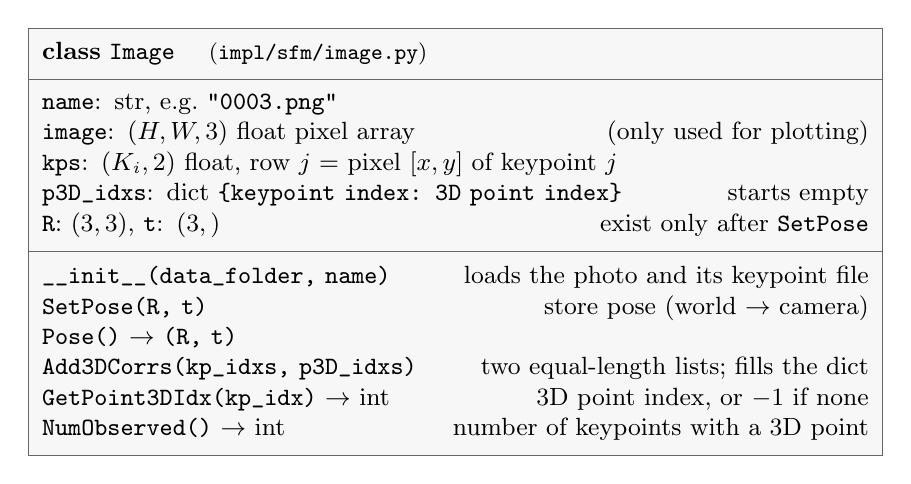
\begin{tikzpicture}
\node[draw=black!60, fill=black!3, rectangle split, rectangle split parts=3,
      text width=10.5cm, font=\small, align=left, inner sep=5pt,
      rectangle split part fill={blue!10,black!3,black!3}] (cls)
{\centering\textbf{class \code{Image}} \quad {\footnotesize(\code{impl/sfm/image.py})}
 \nodepart{second}
 \code{name}: str, e.g.\ \code{"0003.png"}\\
 \code{image}: $(H,W,3)$ float pixel array \hfill (only used for plotting)\\
 \code{kps}: $(K_i, 2)$ float, row $j$ = pixel $[x, y]$ of keypoint $j$\\
 \code{p3D_idxs}: dict \code{{keypoint index: 3D point index}} \hfill starts empty\\
 \code{R}: $(3,3)$, \code{t}: $(3,)$ \hfill exist only after \code{SetPose}
 \nodepart{third}
 \code{__init__(data_folder, name)} \hfill loads the photo and its keypoint file\\
 \code{SetPose(R, t)} \hfill store pose (world $\to$ camera)\\
 \code{Pose()} $\to$ \code{(R, t)}\\
 \code{Add3DCorrs(kp_idxs, p3D_idxs)} \hfill two equal-length lists; fills the dict\\
 \code{GetPoint3DIdx(kp_idx)} $\to$ int \hfill 3D point index, or $-1$ if none\\
 \code{NumObserved()} $\to$ int \hfill number of keypoints with a 3D point};
\end{tikzpicture}
\end{center}

\textbf{Note:} \code{t} must be a flat vector of shape $(3,)$, not $(3,1)$.
\code{TriangulatePoints} calls \code{np.expand_dims(t, 1)} itself.

% =====================================================================
\clearpage
\section{How the data structures point at each other}

This is the part the handout leaves implicit. Everything is connected through
\textbf{integer indices}:

\begin{itemize}
  \setlength{\itemsep}{1pt}
  \item A \textbf{keypoint index} is a row number in \code{image.kps}.
  \item A \textbf{match} is a row \code{[i, j]} of \code{matches[(n1, n2)]}: keypoint $i$ in
        image \code{n1} and keypoint $j$ in image \code{n2} show the same physical point.
        Keys are always sorted (\code{n1 < n2}); \code{GetPairMatches(a, b, matches)} flips
        the columns if you ask for the pair in the other order.
  \item A \textbf{3D point index} is a row number in the global \code{points3D} array.
  \item \code{image.p3D_idxs} links the two: keypoint index $\to$ 3D point index.
\end{itemize}

\begin{figure}[h!]
\centering
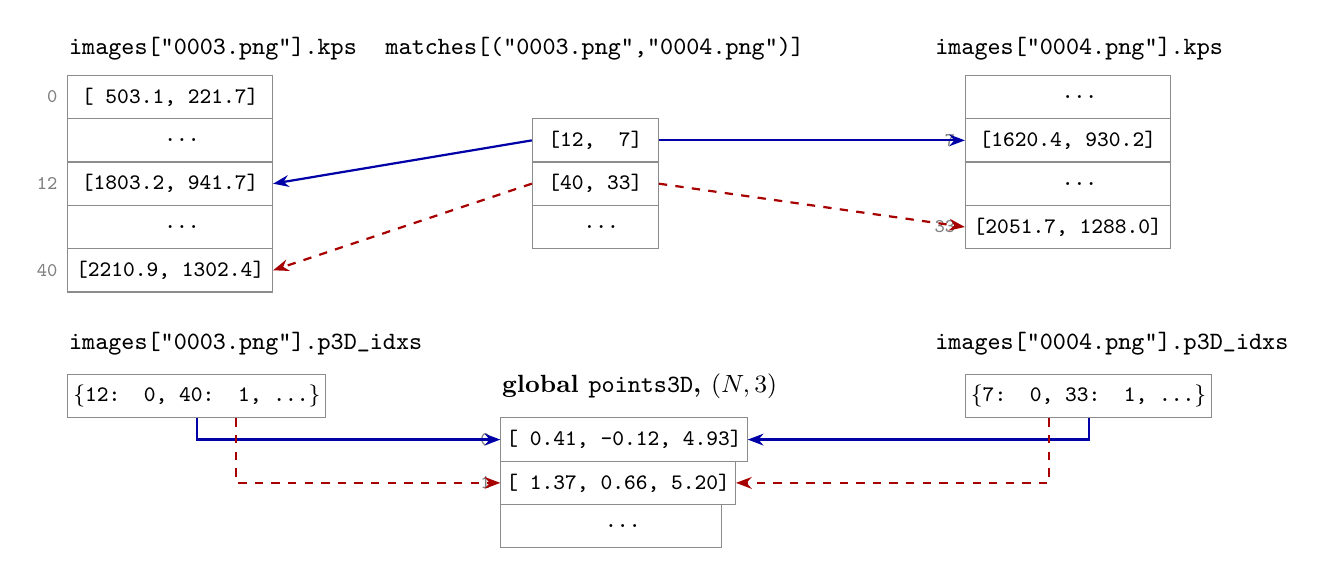
\begin{tikzpicture}[
  cell/.style={draw=black!45, fill=white, minimum height=5.5mm, font=\footnotesize\ttfamily,
               inner sep=2pt, anchor=west},
  hdr/.style={font=\small\bfseries, anchor=south west},
  idx/.style={font=\scriptsize\ttfamily, text=black!50, anchor=east},
  la/.style={-{Stealth[length=2mm]}, thick, blue!65!black},
  lb/.style={-{Stealth[length=2mm]}, thick, red!65!black, dashed}]

% Image A kps
\node[hdr] at (-0.1,0.35) {\code{images["0003.png"].kps}};
\node[cell, minimum width=2.6cm] (ak0) at (0,0)     {[ 503.1,  221.7]};
\node[cell, minimum width=2.6cm] (ak1) at (0,-0.55) {\ \ \dots};
\node[cell, minimum width=2.6cm] (ak2) at (0,-1.1)  {[1803.2,  941.7]};
\node[cell, minimum width=2.6cm] (ak3) at (0,-1.65) {\ \ \dots};
\node[cell, minimum width=2.6cm] (ak4) at (0,-2.2)  {[2210.9, 1302.4]};
\node[idx] at (ak0.west) {0}; \node[idx] at (ak2.west) {12}; \node[idx] at (ak4.west) {40};

% matches
\node[hdr, anchor=south] at (6.7,0.35) {\code{matches[("0003.png","0004.png")]}};
\node[cell, minimum width=1.6cm] (m0) at (5.9,-0.55) {[12,\ \ 7]};
\node[cell, minimum width=1.6cm] (m1) at (5.9,-1.1)  {[40,\ 33]};
\node[cell, minimum width=1.6cm] (m2) at (5.9,-1.65) {\ \dots};


% Image B kps
\node[hdr] at (10.9,0.35) {\code{images["0004.png"].kps}};
\node[cell, minimum width=2.6cm] (bk0) at (11.4,0)     {\ \ \dots};
\node[cell, minimum width=2.6cm] (bk1) at (11.4,-0.55) {[1620.4,  930.2]};
\node[cell, minimum width=2.6cm] (bk2) at (11.4,-1.1)  {\ \ \dots};
\node[cell, minimum width=2.6cm] (bk3) at (11.4,-1.65) {[2051.7, 1288.0]};
\node[idx] at (bk1.west) {7}; \node[idx] at (bk3.west) {33};

\draw[la] (m0.west) -- (ak2.east);
\draw[la] (m0.east) -- (bk1.west);
\draw[lb] (m1.west) -- (ak4.east);
\draw[lb] (m1.east) -- (bk3.west);

% p3D_idxs dicts
\node[hdr] at (-0.1,-3.4) {\code{images["0003.png"].p3D_idxs}};
\node[cell, minimum width=2.6cm] (ad) at (0,-3.8) {\{12: 0,\ 40: 1, \dots\}};
\node[hdr] at (10.9,-3.4) {\code{images["0004.png"].p3D_idxs}};
\node[cell, minimum width=2.6cm] (bd) at (11.4,-3.8) {\{7: 0,\ 33: 1, \dots\}};

% points3D
\node[hdr] at (5.4,-3.95) {global \code{points3D}, $(N,3)$};
\node[cell, minimum width=2.8cm] (p0) at (5.5,-4.35) {[ 0.41, -0.12, 4.93]};
\node[cell, minimum width=2.8cm] (p1) at (5.5,-4.9)  {[ 1.37,  0.66, 5.20]};
\node[cell, minimum width=2.8cm] (p2) at (5.5,-5.45) {\ \ \dots};
\node[idx] at (p0.west) {0}; \node[idx] at (p1.west) {1};

\draw[la] (ad.south) |- (p0.west);
\draw[la] (bd.south) |- (p0.east);
\draw[lb] ($(ad.south)+(0.5,0)$) |- (p1.west);
\draw[lb] ($(bd.south)+(-0.5,0)$) |- (p1.east);
\end{tikzpicture}
\caption{Two example correspondences (blue and red). The first match row says keypoint 12 in 0003
and keypoint 7 in 0004 are the same point. After triangulation, both images' \code{p3D_idxs}
send that keypoint to row 0 of \code{points3D}. Numbers are illustrative.}
\label{fig:indices}
\end{figure}

\textbf{Why this matters.} \code{Find2D3DCorrespondences} walks exactly this chain:
new image keypoint $\xrightarrow{\text{match}}$ registered image keypoint
$\xrightarrow{\text{p3D\_idxs}}$ 3D point. If \code{p3D_idxs} holds wrong indices (e.g.\ local
instead of global in Task 1.5), new images get registered against the wrong 3D points.

% =====================================================================
\section{Zoom-in on each task}

\subsection*{Task 1.1 -- \texttt{EstimateEssentialMatrix(K, im1, im2, matches)} \hfill \normalfont\small\code{geometry.py}}
\begin{center}
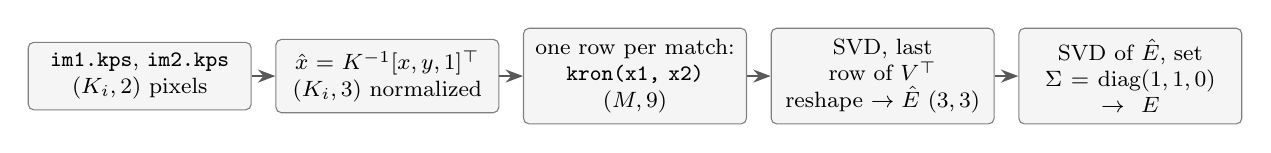
\begin{tikzpicture}[node distance=3mm, s/.style={fn, text width=2.55cm, align=center, font=\footnotesize}]
\node[s] (s1) {\code{im1.kps}, \code{im2.kps}\\ $(K_i,2)$ pixels};
\node[s, right=of s1] (s2) {$\hat{x} = K^{-1}[x, y, 1]^\top$\\ $(K_i,3)$ normalized};
\node[s, right=of s2] (s3) {one row per match:\\ \code{kron(x1, x2)}\\ $(M,9)$};
\node[s, right=of s3] (s4) {SVD, last row of $V^\top$\\ reshape $\to \hat{E}$ $(3,3)$};
\node[s, right=of s4] (s5) {SVD of $\hat{E}$, set\\ $\Sigma = \text{diag}(1,1,0)$\\ $\to E$};
\draw[arr] (s1)--(s2); \draw[arr] (s2)--(s3); \draw[arr] (s3)--(s4); \draw[arr] (s4)--(s5);
\end{tikzpicture}
\end{center}
Ends with an \code{assert} that $|\hat{x}_1^\top E\, \hat{x}_2| < 0.01$ for every match.

\subsection*{Task 1.2 -- \texttt{TriangulatePoints(K, im1, im2, matches)} \hfill \normalfont\small\code{geometry.py}}
Requires both images to have a pose already.
\begin{center}
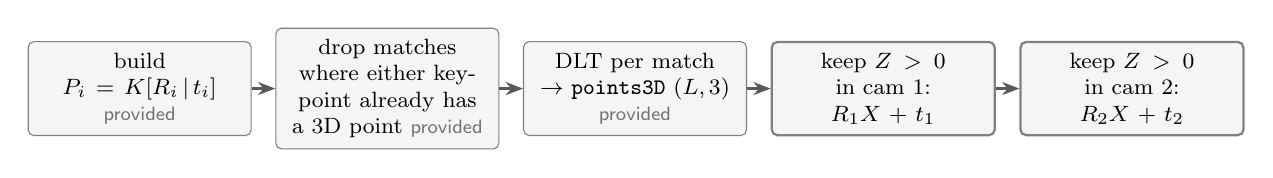
\begin{tikzpicture}[node distance=3mm, s/.style={fn, text width=2.55cm, align=center, font=\footnotesize}]
\node[s] (s1) {build $P_i = K[R_i\,|\,t_i]$\\ \given};
\node[s, right=of s1] (s2) {drop matches where either keypoint already has a 3D point \given};
\node[s, right=of s2] (s3) {DLT per match\\ $\to$ \code{points3D} $(L,3)$\\ \given};
\node[todo, s, right=of s3] (s4) {keep $Z>0$ in cam 1:\\ $R_1X + t_1$};
\node[todo, s, right=of s4] (s5) {keep $Z>0$ in cam 2:\\ $R_2X + t_2$};
\draw[arr] (s1)--(s2); \draw[arr] (s2)--(s3); \draw[arr] (s3)--(s4); \draw[arr] (s4)--(s5);
\end{tikzpicture}
\end{center}
Returns \code{points3D} $(L,3)$, \code{im1_corrs} $(L,)$, \code{im2_corrs} $(L,)$: row $k$ of
each belongs to the same point. Use \textbf{one mask} for all three arrays.

\subsection*{Task 1.3 -- choosing the pose \hfill \normalfont\small\code{sfm.py}}
\textbf{Convention.} The decomposition returns $(R, t)$ with $x_{\text{cam1}} = R\,x_{\text{cam2}} + t$.
\code{SetPose} wants world $\to$ camera, and the world frame is camera 1. So:
\[
  \text{camera 1: } (I,\ \mathbf{0}) \qquad\quad
  \text{camera 2: } (R^\top,\ -R^\top t)
\]
Try all four candidates, call \code{TriangulatePoints} for each, and keep the one returning the
most points. Then set that pose for real; the provided code triangulates once more and calls
\code{Add3DCorrs} with indices \code{0..N-1}.

\subsection*{Task 1.4 -- \texttt{EstimateImagePose(points2D, points3D, K)} \hfill \normalfont\small\code{geometry.py}}
Inputs are $C$ matched pairs: \code{points2D} $(C,2)$ pixels and \code{points3D} $(C,3)$.
Only the normalization is missing. With $\hat{x} = K^{-1}x$, the projection becomes
$\hat{x} \sim [R\,|\,t]X$, so DLT solves for $[R\,|\,t]$ directly. The provided code then
extracts $R$ (closest rotation) and $t$ (from the camera centre).
\code{BuildProjectionConstraintMatrix} only reads columns 0 and 1 of the 2D points.

\subsection*{Task 1.5 -- \texttt{TriangulateImage} + \texttt{UpdateReconstructionState}}

\begin{figure}[h!]
\centering
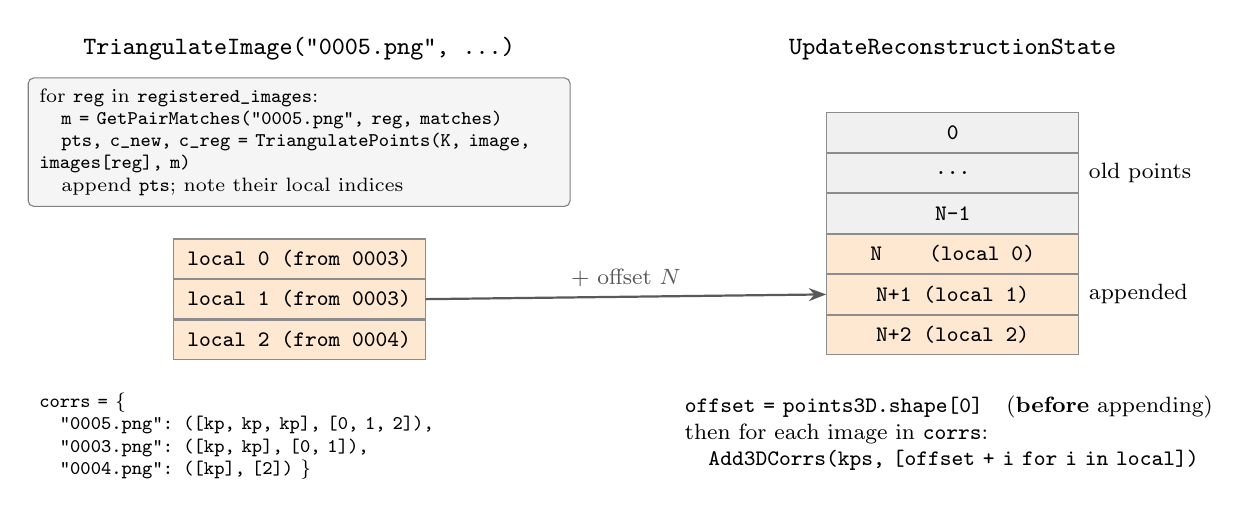
\begin{tikzpicture}[
  row/.style={draw=black!45, minimum width=3.2cm, minimum height=5mm, font=\footnotesize\ttfamily, inner sep=1pt},
  oldrow/.style={row, fill=black!6},
  newrow/.style={row, fill=orange!18}]

% left: TriangulateImage
\node[font=\small\bfseries, anchor=south] at (0,0.4) {\code{TriangulateImage("0005.png", ...)}};
\node[fn, text width=6.6cm, font=\scriptsize, anchor=north] (loop) at (0,0.3)
  {for \code{reg} in \code{registered_images}:\\
   \quad \code{m = GetPairMatches("0005.png", reg, matches)}\\
   \quad \code{pts, c_new, c_reg = TriangulatePoints(K, image, images[reg], m)}\\
   \quad append \code{pts}; note their local indices};
\node[newrow, below=4mm of loop] (l0) {local 0 (from 0003)};
\node[newrow, below=0mm of l0] (l1) {local 1 (from 0003)};
\node[newrow, below=0mm of l1] (l2) {local 2 (from 0004)};
\node[font=\scriptsize\ttfamily, text width=6.6cm, align=left, below=3mm of l2] (cd)
  {corrs = \{\\
   \quad "0005.png": ([kp, kp, kp], [0, 1, 2]),\\
   \quad "0003.png": ([kp, kp], [0, 1]),\\
   \quad "0004.png": ([kp], [2]) \}};

% right: Update
\node[font=\small\bfseries, anchor=south] at (8.3,0.4) {\code{UpdateReconstructionState}};
\node[oldrow] (g0) at (8.3,-0.4) {0};
\node[oldrow, below=0mm of g0] (g1) {\dots};
\node[oldrow, below=0mm of g1] (g2) {N-1};
\node[newrow, below=0mm of g2] (g3) {N\ \ \ \ (local 0)};
\node[newrow, below=0mm of g3] (g4) {N+1 (local 1)};
\node[newrow, below=0mm of g4] (g5) {N+2 (local 2)};
\node[font=\footnotesize, anchor=west] at (g1.east) {old points};
\node[font=\footnotesize, anchor=west] at (g4.east) {appended};
\node[font=\footnotesize, text width=6.8cm, align=left, below=4mm of g5]
  {\code{offset = points3D.shape[0]}\quad (\textbf{before} appending)\\
   then for each image in \code{corrs}:\\
   \quad \code{Add3DCorrs(kps, [offset + i for i in local])}};

\draw[arr] (l1.east) -- node[above, font=\footnotesize]{+ offset $N$} (g4.west);
\end{tikzpicture}
\caption{\code{TriangulateImage} numbers new points from 0. \code{UpdateReconstructionState}
puts them at the end of the global array, so every local index is shifted by the old point count $N$.}
\end{figure}

The new image takes part in every pair, so its entry in \code{corrs} must \emph{grow} across
the loop rather than be overwritten.

% =====================================================================
\clearpage
\section{Function reference}

\renewcommand{\arraystretch}{1.25}
\footnotesize

\subsection*{\texttt{impl/sfm/io.py} and \texttt{impl/util.py} -- loading and coordinate helpers}
\begin{tabularx}{\textwidth}{@{}>{\raggedright\arraybackslash}p{3.6cm} >{\raggedright\arraybackslash}X >{\raggedright\arraybackslash}X >{\raggedright\arraybackslash}p{4.2cm}@{}}
\toprule
\textbf{Function} & \textbf{Input} & \textbf{Output} & \textbf{What it does}\\
\midrule
\code{ReadFeatureMatches} & \code{image_pair} (n1, n2) with n1 < n2; \code{data_folder} & $(M,2)$ int array & reads \code{matches/n1-n2.txt}\\
\code{ReadKMatrix} & \code{data_folder} & \code{K} $(3,3)$ & reads \code{images/K.txt}\\
\code{MakeHomogeneous} & \code{pts}, \code{ax} & same array with a row/column of 1s appended & $[x,y] \to [x,y,1]$. Points in rows $\Rightarrow$ \code{ax=1}\\
\code{HNormalize} & \code{pts}, \code{ax} & divides by last coordinate and drops it & $[x,y,w] \to [x/w, y/w]$\\
\bottomrule
\end{tabularx}

\subsection*{\texttt{impl/sfm/corrs.py} -- bookkeeping between images and 3D points}
\begin{tabularx}{\textwidth}{@{}>{\raggedright\arraybackslash}p{3.6cm} >{\raggedright\arraybackslash}X >{\raggedright\arraybackslash}X >{\raggedright\arraybackslash}p{4.2cm}@{}}
\toprule
\textbf{Function} & \textbf{Input} & \textbf{Output} & \textbf{What it does}\\
\midrule
\code{GetPairMatches} & names \code{im1}, \code{im2}; \code{matches} dict & $(M,2)$: col 0 = keypoint in \code{im1}, col 1 = in \code{im2} & looks up the pair in either order, flipping columns if needed\\
\code{Find2D3DCorrespondences} & new image name, \code{images}, \code{matches}, \code{registered_images} & \code{image_kp_idxs}, \code{p3D_idxs}: lists, length $C$ & follows matches into registered images that already have 3D points; one entry per unique 3D point\\
\code{UpdateReconstruction}\newline\code{State} \textcolor{tododraw}{\bfseries Task 1.5} & \code{new_points3D} $(L,3)$, \code{corrs} dict, \code{points3D} $(N,3)$, \code{images} & \code{points3D} $(N{+}L,3)$, \code{images} & appends points, shifts local $\to$ global indices, calls \code{Add3DCorrs}\\
\bottomrule
\end{tabularx}

\subsection*{\texttt{impl/sfm/geometry.py} and \texttt{impl/dlt.py} -- the geometry}
\begin{tabularx}{\textwidth}{@{}>{\raggedright\arraybackslash}p{3.6cm} >{\raggedright\arraybackslash}X >{\raggedright\arraybackslash}X >{\raggedright\arraybackslash}p{4.2cm}@{}}
\toprule
\textbf{Function} & \textbf{Input} & \textbf{Output} & \textbf{What it does}\\
\midrule
\code{EstimateEssentialMatrix} \newline\textcolor{tododraw}{\bfseries Task 1.1} & \code{K}, \code{im1}, \code{im2} (\code{Image}), \code{matches} $(M,2)$ & \code{E} $(3,3)$ & 8-point DLT on normalized keypoints, then enforce singular values $(1,1,0)$\\
\code{DecomposeEssentialMatrix} & \code{E} & list of 4 \code{(R, t)} & two rotations $\times$ two translation signs (cam 2 $\to$ cam 1)\\
\code{TriangulatePoints} \newline\textcolor{tododraw}{\bfseries Task 1.2} & \code{K}, \code{im1}, \code{im2} \emph{with poses set}, \code{matches} & \code{points3D} $(L,3)$, \code{im1_corrs} $(L,)$, \code{im2_corrs} $(L,)$ & DLT triangulation of not-yet-triangulated matches; removes points behind either camera\\
\code{EstimateImagePose} \newline\textcolor{tododraw}{\bfseries Task 1.4} & \code{points2D} $(C,2)$ px, \code{points3D} $(C,3)$, \code{K} & \code{R} $(3,3)$, \code{t} $(3,)$ & absolute pose by DLT on normalized points\\
\code{TriangulateImage} \newline\textcolor{tododraw}{\bfseries Task 1.5} & \code{K}, new \code{image_name}, \code{images}, \code{registered_images}, \code{matches} & new points $(L,3)$ (local idx), \code{corrs} dict & triangulates new image against every registered image\\
\code{BuildProjection}\newline\code{ConstraintMatrix} & \code{points2D} $(C,\ge2)$, \code{points3D} $(C,3)$ & $(2C,12)$ & two DLT rows per 2D--3D pair (\code{dlt.py})\\
\bottomrule
\end{tabularx}

\subsection*{\texttt{impl/sfm/vis.py} and \texttt{impl/vis.py} -- plotting (all provided)}
\begin{tabularx}{\textwidth}{@{}>{\raggedright\arraybackslash}p{3.6cm} >{\raggedright\arraybackslash}X >{\raggedright\arraybackslash}X >{\raggedright\arraybackslash}p{4.2cm}@{}}
\toprule
\textbf{Function} & \textbf{Input} & \textbf{Output} & \textbf{What it does}\\
\midrule
\code{PlotImages} & \code{images} dict & figure & grid of all photos\\
\code{PlotWithKeypoints} & one \code{Image} & figure & photo with red keypoints\\
\code{PlotImagePairMatches} & \code{im1}, \code{im2}, \code{matches} & figure (\textbf{blocking}) & side-by-side photos with green match lines; 45 windows in \code{sfm.py}\\
\code{PlotCameras} & \code{images}, \code{registered_images}, \code{ax} & draws on \code{ax} & calls \code{PlotCamera} for each registered image\\
\code{Plot3DPoints} & \code{points} $(N,3)$, \code{ax} & \code{ax} & black dots for the point cloud\\
\code{PlotCamera} & \code{R}, \code{t}, \code{ax}, \code{scale}, \code{color} & \code{ax} & camera frustum at centre $-R^\top t$\\
\bottomrule
\end{tabularx}

\normalsize

% =====================================================================
\section{Conventions to keep straight}
\begin{itemize}
  \setlength{\itemsep}{2pt}
  \item \textbf{Pose} \code{(R, t)} in an \code{Image} maps \emph{world} $\to$ \emph{camera}:
        $X_{\text{cam}} = R X_{\text{world}} + t$. The camera centre is $-R^\top t$.
  \item \textbf{World frame} = camera of image 0003 (identity pose).
  \item \textbf{Essential matrix}: $\hat{x}_1^\top E\, \hat{x}_2 = 0$ (image 1 on the left),
        matching the \code{assert}.
  \item \textbf{Depth test}: a point is in front of a camera if $Z > 0$ after
        $R X + t$.
  \item \textbf{Normalized coordinates}: $\hat{x} = K^{-1}[u, v, 1]^\top$, the viewing-ray
        direction with the camera's internal parameters removed.
  \item \textbf{Array layout}: one point per \emph{row} everywhere (\code{kps}, \code{points3D},
        matches), so use \code{ax=1} with the \code{util.py} helpers and transpose around
        matrix products: \code{(A @ pts.T).T}.
\end{itemize}

% =====================================================================
\section{Part 2: \texttt{line\_fitting.py}}

\begin{figure}[h!]
\centering
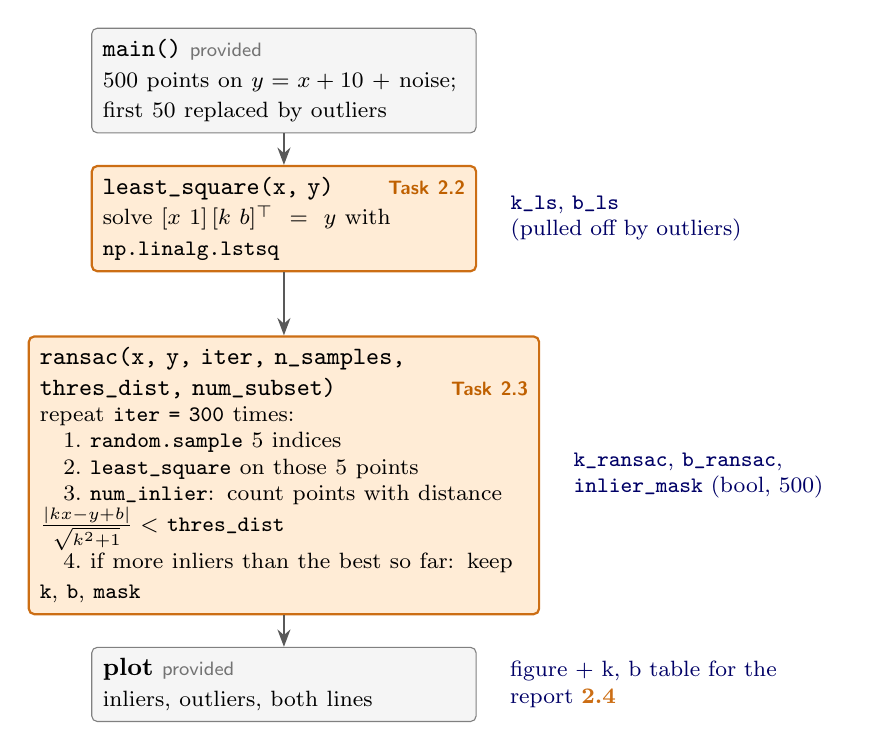
\begin{tikzpicture}[node distance=4mm]
\node[fn, text width=4.6cm] (g) {\fnn{main()} \given\\ {\footnotesize 500 points on $y = x + 10$ + noise; first 50 replaced by outliers}};
\node[todo, text width=4.6cm, below=of g] (ls) {\fnn{least_square(x, y)} \task{2.2}\\ {\footnotesize solve $[x\ 1]\,[k\ b]^\top = y$ with \code{np.linalg.lstsq}}};
\node[outn, text width=3.6cm, right=3mm of ls] {\code{k_ls}, \code{b_ls}\\ (pulled off by outliers)};

\node[todo, text width=6.2cm, below=8mm of ls] (r) {\fnn{ransac(x, y, iter, n_samples, thres_dist, num_subset)} \task{2.3}\\
  {\footnotesize repeat \code{iter = 300} times:\\
  \quad 1.\ \code{random.sample} 5 indices\\
  \quad 2.\ \code{least_square} on those 5 points\\
  \quad 3.\ \fnn{num_inlier}: count points with distance $\frac{|kx - y + b|}{\sqrt{k^2+1}} <$ \code{thres_dist}\\
  \quad 4.\ if more inliers than the best so far: keep \code{k}, \code{b}, \code{mask}}};
\node[outn, text width=3.6cm, right=3mm of r] {\code{k_ransac}, \code{b_ransac}, \code{inlier_mask} (bool, 500)};

\node[fn, text width=4.6cm, below=of r] (p) {\textbf{plot} \given\\ {\footnotesize inliers, outliers, both lines}};
\node[outn, text width=3.6cm, right=3mm of p] {figure + k, b table for the report \textcolor{tododraw}{\bfseries 2.4}};

\draw[arr] (g) -- (ls); \draw[arr] (ls) -- (r); \draw[arr] (r) -- (p);
\end{tikzpicture}
\end{figure}

\end{document}
